\subsubsection{BaseBubble}

\label{BaseBubble}
\begin{figure}[ht]
	\centering
	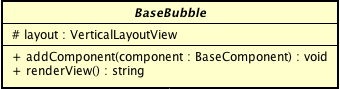
\includegraphics[scale=0.5]{Sezioni/SottosezioniST/img/BaseBubble.png}
	\caption{BaseBubble}
\end{figure}

\begin{itemize}
\item \textbf{Descrizione:} Classe base astratta che rappresenta le bolle di Monolith.
\item \textbf{Utilizzo:} Classe base astratta utilizzata ed estesa ogni qualvolta uno sviluppatore intende creare nuove bolle.
\item \textbf{Attributi:} 
\begin{itemize}
\item \textit{protected layout:VerticalLayoutView}\\
Oggetto che rappresenta il layout verticale della bolla.
\end{itemize}
\item \textbf{Metodi:}
\begin{itemize}
\item \textit{public addWidget(widget:BaseWidgetView):void}\\
Aggiunge un widget alla bolla.
\item{\textbf{Parametri}: \begin{itemize}
\item \textit{widget:BaseWidgetView}\\
Oggetto che rappresenta il widget che si desidera aggiungere alla bolla.
\end{itemize}}
\item \textit{public addLayout(layout:BaseLayoutView):void}\\
Aggiunge un layout alla bolla.
\item{\textbf{Parametri}: \begin{itemize}
\item \textit{layout:BaseLayoutView}\\
Oggetto che rappresenta il layout che si desidera aggiungere alla bolla.
\end{itemize}}
\item \textit{public renderView():string}\\
Genera il codice HTML, CSS e JavaScript necessario per visualizzare bolle.
\end{itemize}
\end{itemize}

\subsubsection{ToDoListBubble}

\label{ToDoListBubble}
\begin{figure}[ht]
	\centering
	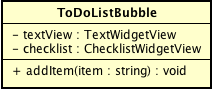
\includegraphics[scale=0.5]{Sezioni/SottosezioniST/img/ToDoListBubble.png}
	\caption{ToDoListBubble}
\end{figure}

\begin{itemize}
\item \textbf{Descrizione:} Classe concreta che estende BaseBubble, destinata alla creazione di bolle lista di Monolith.
\item \textbf{Utilizzo:} Classe utilizzata ogni qualvolta uno sviluppatore intende creare nuove bolle lista.
\item \textbf{Attributi:}
\begin{itemize}
\item \textit{private textView:TextWidgetView}\\
Oggetto che rappresenta il widget contenente il testo della bolla lista.
\item \textit{private checklistView:CheckListView}\\
Oggetto che rappresenta il widget contenente la lista di oggetti che si possono spuntare.
\end{itemize}
\item \textbf{Metodi:}
\begin{itemize}
\item \textit{public addItem(item:string):void}\\
Aggiunge un elemento con il nome definito alla bolla lista.
\item{\textbf{Parametri}: \begin{itemize}
\item \textit{item:string}\\
Valore che rappresenta il nome dell'elemento che si vuole aggiungere alla lista.
\end{itemize}}
\end{itemize}
\end{itemize}

\subsubsection{MarkdownBubble}

\label{MarkdownBubble}
\begin{figure}[ht]
	\centering
	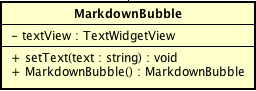
\includegraphics[scale=0.5]{Sezioni/SottosezioniST/img/MarkdownBubble.png}
	\caption{MarkDownBubble}
\end{figure}

\begin{itemize}
\item \textbf{Descrizione:} Classe concreta che estende BaseBubble, destinata alla creazione di bolle testo markdown di Monolith.
\item \textbf{Utilizzo:} Classe utilizzata ogni qualvolta uno sviluppatore intende creare nuove bolle testo markdown.
\item \textbf{Attributi:}
\begin{itemize}
\item \textit{private textview:TextWidgetView}\\
Oggetto che rappresenta il widget contenente il testo della bolla testo markdown.
\end{itemize}
\item \textbf{Metodi:}
\begin{itemize}
\item \textit{public setText(text:string):void}\\
Imposta il testo della bolla lista con il valore definito.
\item{\textbf{Parametri}: \begin{itemize}
\item \textit{text:string}\\
Valore che rappresenta il testo che si vuole inserire nella bolla testo markdown.
\end{itemize}}
\end{itemize}
\end{itemize}

\subsubsection{AlertBubble}

\label{AlertBubble}
\begin{figure}[ht]
	\centering
	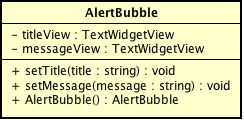
\includegraphics[scale=0.5]{Sezioni/SottosezioniST/img/AlertBubble.png}
	\caption{AlertBubble}
\end{figure}

\begin{itemize}
\item \textbf{Descrizione:} Classe concreta che estende BaseBubble, destinata alla creazione di bolle avviso di Monolith.
\item \textbf{Utilizzo:} Classe utilizzata ogni qualvolta uno sviluppatore intende creare nuove bolle avviso.
\item \textbf{Attributi:} 
\begin{itemize}
\item \textit{private titleView:TextWidgetView}\\
Campo che rappresenta e contiene il titolo della bolla avviso.
\item \textit{private messageView:TextWidgetView}\\
Campo che rappresenta e contiene il messaggio della bolla avviso.
\end{itemize}
\item \textbf{Metodi:}
\begin{itemize}
\item \textit{public setTitle(title:string):void}\\
Imposta il titolo della bolla avviso con il valore title.
\item{\textbf{Parametri}: \begin{itemize}
\item \textit{title:string}\\
Valore che rappresenta il titolo che si vuole impostare alla bolla avviso.
\end{itemize}}
\item \textit{public setMessage(message:string):void}\\
Imposta il messaggio della bolla avviso con il valore message.
\item{\textbf{Parametri}: \begin{itemize}
\item \textit{message:string}\\
Valore che rappresenta il messaggio testuale che si vuole impostare alla bolla avviso.
\end{itemize}}
\end{itemize}
\end{itemize}